\section{React Native}
\label{sec:Frameorks_ReactNative}

Das von Meta, ehemals Facebook, entwickelte React Native Framework ermöglicht die Cross-Plattform Entwicklung mit Webtechnologien.
Dabei kommt die verbreitete \ac{UI}-Bibliothek React zum Einsatz, um die Benutzeroberfläche zu erstellen.
Als Zielplattformen werden neben Android und iOS unter anderem Windows und macOS unterstützt \cite{ReactNative}.
Ein großer Vorteil des Frameworks ist die Verwendung von React für die Umsetzung der \ac{UI}.
Da viele Webentwickler mit React vertraut sind, fällt die Einarbeitung in React Native leicht, was zu einer großen Verbreitung des Frameworks führt \cite{Appfigures_TopSDKs,Stackoverflow_2022}.
Außerdem lässt sich React Native vergleichsweise einfach in bestehende native Projekte integrieren, was die inkrementelle Migration von Projekten ermöglicht.
Diese Integrationsmöglichkeit führt auch dazu, dass neben den Apps von Meta, weitere populäre Apps wie die Microsoft Office Apps, Pinterest und WordPress teile ihrer Funktionalität mit React Native umsetzen \cite{ReactNative_Showcase}.


Obwohl React Native wie Cordova und Capacitor auf Webtechnologien, insbesondere JavaScript, basiert, wählt das Framework einen anderen Ansatz, um die Cross-Plattform Entwicklung zu ermöglichen.
Mit Ionic können Cordova und Capacitor Apps ebenfalls React als \ac{UI}-Bibliothek verwenden.
Dabei ist die Oberfläche komplett als Webanwendung implementiert und wird in einer WebView der jeweiligen Plattform dargestellt.
ReactNative verzichtet hingegen auf den Einsatz einer WebView und nutzt stattdessen die nativen \ac{UI}-Komponenten der jeweiligen Plattformen.
Der JavaScript Code wird nicht, wie bei Foreign Language Apps nach Nunkesser \cite{Nunkesser_Taxonomy_Apps}, in nativ ausführbaren Code übersetzt, sondern in einer JavaScript-Runtime ausgeführt.
Somit lässt sich  React Native weder komplett den Hybrid Web Apps noch den Foreign Language Apps zuordnen.
Stattdessen handelt es sich um Hybrid Bridged Apps, da Webtechnologien und native \ac{UI}-Elemente in einer App kombiniert werden.


Aktuell wird die Architektur von React Native auf einen neuen Ansatz umgestellt, der Probleme der bisherigen Architektur beheben soll.
Da jedoch noch beide Ansätze unterstützt werden, wird hier sowohl auf die bisherige als auch auf die neue Architektur eingegangen.

Die bisherige Architektur setzt sich aus zwei Komponenten zusammen, welche über die sogenannte React Native Bridge miteinander kommunizieren.
Die Bridge trennt dabei JavaScript von der nativen Umgebung.
Der JavaScript-Code innerhalb der JavaScriptCore Ausführungsumgebung, einem Teil der Open-Source Browser Engine WebKit, ausgeführt.
JavaScriptCore läuft in einem eigenen Thread, der wegen der Ausführung von JavaScript innerhalb der Ausführungsumgebung auch als JavaScript-Thread oder kurz JS-Thread bezeichnet wird.
Unter iOS ist die WebKit Engine Teil des Betriebssystems und wird von Apple bereitgestellt.
Alle React Native-Apps können die vorhandene Engine nutzen und müssen diese nicht mitliefern.
Android stellt JavaScriptCore nicht bereit, weshalb ReactNative-Apps für Android JavaScriptCore mitliefern müssen und demnach größer ausfallen \cite{Dragomir_ReactNative,Nawrocki_Comparison_Hybrid_Native_Frameworks}.
Die \ac{UI} wird von der nativen Umgebung, dem sogenannten nativen Thread, gerendert.
Die Bridge übernimmt im Wesentlichen die Kommunikation zwischen den beiden Threads, welche in \autoref{fig:reactnative_bridge} schematisch dargestellt ist.
Jegliche Kommunikation zwischen den Threads ist dabei immer asynchron \cite{ReactNative_newArchitecture}.
Render-Anweisungen werden vom JS-Thread an den nativen Thread gesendet und umgekehrt werden Eingaben und Events vom nativen Thread an den JS-Thread übermittelt.
Die Kommunikation erfolgt über Nachrichten, welche im \ac{JSON} Format serialisiert übertragen werden \cite{Dragomir_ReactNative}.
\begin{figure}[ht]
  \centering
  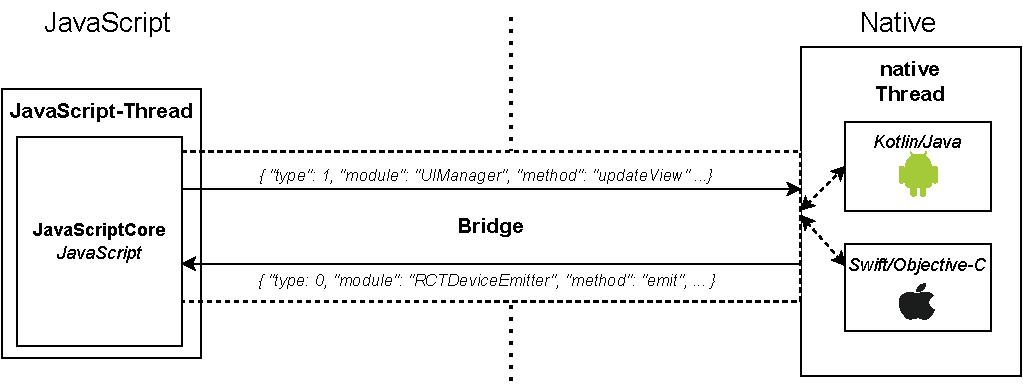
\includegraphics[width=0.85\textwidth]{reactnative_bridge.pdf}
  \caption{Austausch von JSON-Nachrichten zwischen JS-Thread und nativem Thread über die  React Native Bridge.}
  \label{fig:reactnative_bridge}
\end{figure}

Aufgrund des hohen Overheads durch die Kommunikation über \ac{JSON}-Nachrichten, kann es bei vielen ausgetauschten Nachrichten zu Performance-Problemen beim Rendern der \ac{UI} kommen.
Zum Beispiel beim Scrollen von Listen oder bei Animationen werden viele Nachrichten zwischen den beiden Threads ausgetauscht.
In der Folge werden neue Listen-Elemente verzögert gerendert und Animationen erreichen durch den Kommunikationsoverhead keine ausreichende Framerate damit sie flüssig wirken \cite{Cook_ReactNativeBridge}.

\begin{figure}[ht]
  \centering
  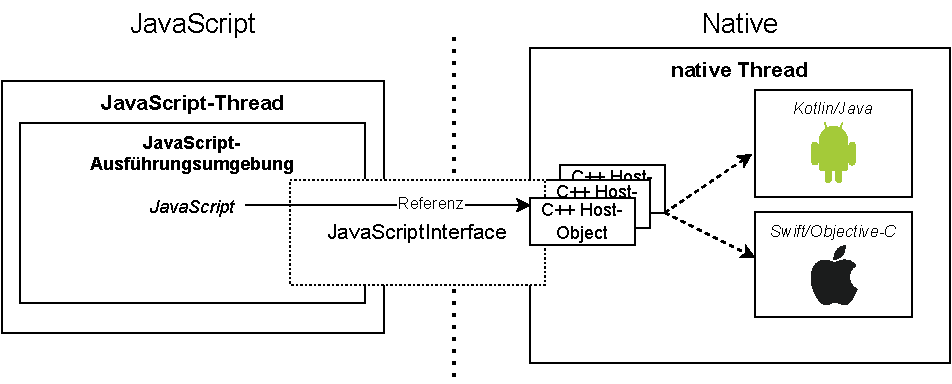
\includegraphics[width=0.85\textwidth]{reactnative_newArchitecture.pdf}
  \caption{Neue Architektur von React Native. Zugriff von JavaScript auf native Host-Objects über das \ac{JSI}.}
  \label{fig:reactnative_newArchitecture}
\end{figure}
Die neue Architektur, dargestellt in \autoref{fig:reactnative_newArchitecture}, soll unter anderem diese Probleme lösen und auch synchrone Kommunikation zwischen den beiden Threads ermöglichen.
Für die Kommunikation von JavaScript mit nativem Code wird die React Native Bridge durch eine neue Schnittstelle das sogenannte \ac{JSI} ersetzt \cite{Cook_ReactNativeBridge}.
Die neue Schnittstelle erlaubt es, in JavaScript-Code Referenzen auf C++-Objekte, sogenannte Host-Objects zu verwenden.
Methoden dieser Objekte können aus JavaScript heraus aufgerufen werden und können JavaScript-Objekte oder weitere Host-Objekte zurückgeben.
Host-Objects können beliebigen C++-Code ausführen oder auch auf Objekte in den nativen Sprachen der Plattform zugreifen \cite{Parashuram_React}.
Dabei ist keine serialisierte Kommunikation mehr notwendig, und die Menge der ausgetauschten Daten kann reduziert werden.
Zum Beispiel beim Anwendungsfall einer Kamerasteuerung, wie in \autoref{fig:reactnative_nativeModules} gezeigt, kann die Aufnahme-Funktion eine Referenz auf ein Bild zurückgeben, anstatt das Bild zu serialisieren und über die Bridge zu übertragen.
Auf dieser Referenz können weitere Funktionen zum Beispiel zur Bearbeitung, aufgerufen werden \cite{Parashuram_React}.
\begin{figure}[ht]
  \centering
  
\includegraphics[width=0.85\textwidth]{reactnative_nativemodules}
  \caption{Vorteile der neuen Architektur für den Zugriff auf native Funktionen \cite{Parashuram_React}.}
  \label{fig:reactnative_nativeModules}  
\end{figure}
Der Aufruf von nativem Code bei React Native ähnelt dem Aufruf von \ac{DOM}-Funktionen durch JavaScript im Browser.
\ac{DOM}-Funktionen können zum Beispiel genutzt werden, um Elemente einer Webseite zu manipulieren.
Dazu greift JavaScript auf Funktionen eines vom Browser bereitgestellten Objekts zu, welche wiederum den zugrundeliegenden nativen Code des Browsers aufrufen \cite{ReactNative_newArchitecture}.
Parashuram \cite{Parashuram_React} bezeichnet den Aufruf von nativer Funktionalität auch als \ac{RPC} zwischen JavaScript und nativem Code.

Die neue Architektur vereinfacht darüber hinaus das Ersetzen der JavaScript Ausführungsumgebung.
Bisher war aufgrund engen Kopplung der Ausführungsumgebung und der Bridge nur JavaScriptCore möglich.
Über einfache Adapter lassen sich neben JavaScriptCore beispielsweise auch die leichtgewichtige, für React Native optimierte Hermes Engine oder Googles V8 Engine verwenden \cite{Cook_ReactNativeBridge,JSI_Adapter}.



Entwickler können eigene sogenannte Turbo Native Modules implementieren, um nativen Code in JavaScript aufrufbar zu machen.
Solche Module sind als Host-Objects im JavaScript-Code verfügbar und beliebige C++-Funktionen können über das \ac{JSI} direkt aus JavaScript aufgerufen werden.
Diese Funktionen können selbst wiederum Funktionen der nativen Programmiersprachen, wie Java oder Objective-C, aufrufen und so zum Beispiel die Kamera-\acp{API} nutzen \cite{Parashuram_React}.
Die Schnittstellen dieser Module zur JavaScript-Seite werden in einer typisierten JavaScript-Variante, beispielsweise TypeScript, definiert.
Damit wird die automatische Codegenerierung des benötigten C++, Java und Objective-C-Code erleichtert, die dem Entwickler die Arbeit zur Definition der Schnittstellen erleichtert \cite{ReactNative_newArchitecture}. 

Durch die Verwendung von nativen \ac{UI}-Elementen ist die Performance von React Native bei \ac{UI}-Operationen vergleichbar mit nativen Apps und besser als hybride Apps mit Cordova oder Capacitor \cite{Huber_UI}.
Ähnlich wie Xamarin unter iOS, fallen React Native Apps unter Android durch die Mitlieferung der JavaScript-Engine vergleichsweise groß aus \cite{Nawrocki_Comparison_Hybrid_Native_Frameworks}.
Durch die neue Architektur und die einfachere Integration anderer JavaScript-Engines, wie Hermes, kann dieses Problem in Zukunft vermutlich gelöst werden.
Abhängig vom Anwendungsfall können sind React Native Apps ähnlich performant wie native Apps oder auch deutlich langsamer \cite{Nawrocki_Comparison_Hybrid_Native_Frameworks}.
Beim Zugriff auf native Funktionen schneidet React Native besser ab als Flutter, Cordova und Capacitor.
Vergleichswerte zu Xamarin fehlen hier jedoch \cite{Biorn-Hansen_PerformanceOverhead_CrossPlatform}.

In der Stackoverflow-Umfrage 2022 \cite{Stackoverflow_2022} geben von allen Entwicklern, welche bereits mit React Native gearbeitet haben, eine Mehrheit von knapp 56 \% an, dass sie das Framework auch weiterhin einsetzen wollen.
Damit schneidet React Native besser ab als Xamarin und Cordova, aber schlechter als Capacitor und Flutter.
Bei Betrachtung der Entwickler, ohne Erfahrung mit dem Framework, welche interessiert daran sind es einzusetzen, liegt React Native jedoch nur knapp hinter dem auch in dieser Kategorie beliebtesten Framework Flutter.